\documentclass{article}

\usepackage{amsmath}
\usepackage{amssymb}
\usepackage{graphicx}
\usepackage[spanish]{babel}
\usepackage{cancel}
\usepackage{enumerate}
\usepackage{hyperref}
\hypersetup{
    colorlinks,
    citecolor=black,
    filecolor=black,
    linkcolor=black,
    urlcolor=black,
}
\usepackage{tcolorbox}
\usepackage{xcolor}

\tcbuselibrary{theorems}

% TODO Remove after completing this document
%\usepackage{caption}
%\usepackage[margin=1.5in]{geometry}
%\usepackage[utf8]{inputenc}
%\usepackage{tcolorbox}
%\usepackage{esint}

\newcommand{\hresult}[2]{\tcboxmath[colback=orange!25!white,colframe=orange, title=#1] {#2} }
\newcommand{\hresulte}[3]{\tcboxmath[colback=orange!25!white,colframe=orange, title=#1] { \hspace{#3} #2 \hspace{#3} } }

\renewcommand{\Bbb}{\mathbb}

\title{Ejercicios de Análisis Matemático CBC (28) \\
Práctica 0: Preliminares \\
Cátedra Ruiz, curso 62802 \\
1° C 2003}
\author{Darío Eduardo Ramos}

\begin{document}
\maketitle

\tableofcontents{}

\newpage

\section*{1}
\label{sec:1}
\addcontentsline{toc}{section}{\nameref{sec:1}}

\textbf{Calcule:}

\begin{enumerate}[(a)]
\bfseries

\item $\frac{2}{3} - \left[ -\frac{1}{2} + 1 - \left( -\frac{1}{2} - \frac{5}{12} \right) - 2  \right] -\frac{1}{4} - \left[ -1 -\left(2 \frac{1}{6} - \frac{1}{4} -\right) +\frac{2}{3} \right]$

\item $\frac{2}{5} + (-2) \left[ -\frac{1}{2} + 1 -\left( \frac{1}{5} -\frac{3}{10} \right) -\frac{1}{4} \right]$

\end{enumerate}
\hrule

\subsection*{1.a}
\label{subsec:1.a}
\addcontentsline{toc}{subsection}{\nameref{subsec:1.a}}

Esto es un simple repaso de aritmética básica. Además de operar con fracciones, tema que se da por conocido, para resolver estos ejercicios es recomendable tener en cuenta lo siguiente:

\begin{itemize}
\item El producto tiene prioridad sobre la suma y la resta. Vale decir, a la hora de evaluar una expresión como $2 \frac{1}{6} - \frac{1}{4}$, primero se evalúa el producto. Por lo tanto, dicha expresión equivale a $\frac{1}{3} - \frac{1}{4}$.

\item Siempre conviene evaluar por completo los paréntesis más anidados e ir progresando hacia afuera.
\end{itemize}

Aplicando estas ideas, se obtiene:

\begin{subequations}
\begin{align}
&\frac{2}{3} - \left[ -\frac{1}{2} + 1 \textcolor{blue}{ \underbrace{ - \left( -\frac{1}{2} - \frac{5}{12} \right)}_{-\left(    -\frac{11}{12} \right)}} - 2  \right] -\frac{1}{4} - \left[ -1 \textcolor{blue}{ \underbrace{ -\left(2 \frac{1}{6} - \frac{1}{4} \right) }_{-\left( \frac{1}{12} \right)}} +\frac{2}{3} \right] = \\
&\frac{2}{3} \underbrace{ - \left[ -\frac{1}{2} + 1 \textcolor{blue}{ + \frac{11}{12} } - 2  \right] }_{\textcolor{red}{-\left[ -\frac{7}{12} \right]}} -\frac{1}{4} \underbrace{-\left[ -1 \textcolor{blue}{ -\frac{1}{12} } +\frac{2}{3} \right]}_{\textcolor{red}{-\left[ -\frac{5}{12} \right]}} = \\ 
&\frac{2}{3} \textcolor{red}{ +\frac{7}{12} } -\frac{1}{4} \textcolor{red}{ +\frac{5}{12} } = \hresult{1.a} { \frac{17}{12} }
\end{align}
\end{subequations}

\subsection*{1.b}
\label{subsec:1.b}
\addcontentsline{toc}{subsection}{\nameref{subsec:1.b}}

Resolviendo con la misma metolodogía que el anterior, se obtiene:

\begin{equation}
\hresult{1.b} { -\frac{3}{10} }
\end{equation}

\section*{2}
\label{sec:2}
\addcontentsline{toc}{section}{\nameref{sec:2}}

\textbf{Calcule:}

\begin{enumerate}[(a)]
\bfseries

\item $\left[ \frac{1}{4} - \left( \frac{2}{3} - \frac{1}{2} \right)^2 \right]^{-2}$

\item $\left[ \left( 4 - \frac{1}{2} \right)^2 + \left( -3-\frac{1}{2} \right)^2 \right]^{\frac{1}{2}}$

\end{enumerate}
\hrule

\subsection*{2.a}
\label{subsec:2.a}
\addcontentsline{toc}{subsection}{\nameref{subsec:2.a}}

El enfoque del punto anterior sigue valiendo, en particular lo referido a evaluar los paréntesis más anidados primero. Lo que se agrega es lidiar con potencias. Y para ello, es conveniente tener presente que:

\begin{itemize}
\item La potenciación no es distributiva respecto a la suma o resta, pero sí respecto al producto.
\begin{itemize}
\renewcommand{\labelitemii}{$\diamond$}
\item $\left(a + b\right)^c \neq a^c + b^c \quad \forall a,b,c \in \mathbb{R}$
\item $\left(a \cdot b\right)^c = a^c \cdot b^c \quad \forall a,b,c \in \mathbb{R}$
\end{itemize}
\item Elevar a una potencia negativa equivale a elevar el recíproco de la misma potencia negada. Simbólicamente, $a^{-b} = \left( \frac{1}{a} \right)^b$, para todo a y b reales, con $a \neq 0$.
\item Elevar a una potencia de la forma $\frac{1}{n}$, con $n$ entero y $n \neq 0$, equivale a tomar la n-ésima raíz de la base: $a^{\frac{1}{n}} = \sqrt[n]{a}$.
\end{itemize}

Aplicando estos conceptos:

\begin{subequations}
\begin{align}
&\left[ \frac{1}{4} - \textcolor{blue}{ \underbrace{ \left( \frac{2}{3} - \frac{1}{2} \right)^2 }_{\left( \frac{1}{6} \right)^2 }} \right]^{-2} = \\
&\left[ \frac{1}{4} - \textcolor{blue}{ \frac{1}{36} } \right]^{-2} = \left[ \frac{8}{36} \right]^{-2} = \left[ \frac{2}{9} \right]^{-2} = \left[ \frac{9}{2} \right]^2 = \hresult{2.a} { \frac{81}{4} = 20.25 }
\end{align}
\end{subequations}

\subsection*{2.b}
\label{subsec:2.b}
\addcontentsline{toc}{subsection}{\nameref{subsec:2.b}}

Es muy similar al anterior, pero se agrega un concepto. Al expresar un resultado, no es deseable que haya expresiones radicales en el denominador. Por ello se entiende raíces de números o expresiones. Para resolver eso, se multiplica y divide por la misma expresión radical a eliminar. En este caso, partiendo del resultado final con expresión radical:

\begin{equation}
\sqrt{\frac{49}{2}} = \frac{7}{\sqrt{2}} = \frac{7}{\sqrt{2}} \frac{\sqrt{2}}{\sqrt{2}} = \hresult{2.b} { \frac{7 \sqrt{2}}{2} \approx 4.9497 }
\end{equation}

\section*{3}
\label{sec:3}
\addcontentsline{toc}{section}{\nameref{sec:3}}

\textbf{Calcule:}

\begin{enumerate}[(a)]
\bfseries

\item $ \frac{3^4 \cdot 3^7}{3^{12}} $

\item $\sqrt{ \frac{ (5 \cdot 10^{-6}) (4 \cdot {10}^2) }{8 \cdot {10}^5} }$

\item $ {81}^{\frac{3}{4}} + \left( \frac{16}{49} \right)^{-\frac{1}{2}} + \left( \frac{64}{27} \right)^{\frac{2}{3}} + {32}^{-\frac{4}{5}} + \left( {{2}^{-6}} \right) ^{\frac{2}{3}} + 3^{\frac{7}{2}} \cdot 3^{\frac{1}{2}} $

\item $ \sqrt{5^2} + \sqrt{(-3)^2} + \sqrt[4]{(-9)^2} + \sqrt[3]{-\frac{8}{27}} + \sqrt[3]{81} $

\end{enumerate}
\hrule

\subsection*{3.a}
\label{subsec:3.a}
\addcontentsline{toc}{subsection}{\nameref{subsec:3.a}}

Al multiplicar potencias de igual base, los exponentes se suman. Y al dividir potencias de igual base, los exponentes se restan.

\begin{itemize}
\item $ a^b \cdot a^c = a^{b + c} \quad \forall a, b, c \in \mathbb{R}$
\item $ \frac{a^b}{a^c} = a^{b - c} \quad \forall a, b, c \in \mathbb{R}$
\end{itemize}

\begin{equation}
\frac{3^4 \cdot 3^7}{3^{12}} = \frac{3^{11}}{3^{12}} = 3^{-1} = \hresulte{3.a} { \frac{1}{3} } {0.25em}
\end{equation}

\subsection*{3.b}
\label{subsec:3.b}
\addcontentsline{toc}{subsection}{\nameref{subsec:3.b}}

En el ejercicio 2.a, se vio cómo lidiar con exponentes de la forma $\frac{1}{n}$, con $n$ entero. Para el caso más general de un exponente fraccionario, puede descomponerse la exponenciación en un paso entero y un paso de la forma $\frac{1}{n}$. Verbigracia:

\begin{equation}
a^{\frac{p}{q}} = a^{(p \frac{1}{q})} = (a^p)^{\frac{1}{q}}
\end{equation}

Así, si resulta conveniente, es posible evaluar $a^p$ primero y luego tomar la q-ésima raíz de ese valor.

Aplicando todo lo ya visto a este caso:

\begin{subequations}
\begin{align}
& \sqrt{ \frac{ (5 \cdot 10^{-6}) (4 \cdot {10}^2) }{8 \cdot {10}^5} } = \\
& \sqrt{ \frac{ 20 \cdot 10^{-4} }{8 \cdot {10}^5} } = \\
& \sqrt{ \frac{5}{2} \cdot 10^{-9} } = \\
& \sqrt{ \frac{5}{2} } \cdot 10^{-\frac{9}{2}} = \\
& \frac{\sqrt{5}}{\sqrt{2}} \cdot \frac{\sqrt{2}}{\sqrt{2}} \cdot 10^{-\frac{9}{2}} = \\
& \frac{\sqrt{10}}{2} \cdot 10^{-4} \cdot 10^{-\frac{1}{2}} = \\
& \frac{1}{2} \cdot \cancel{10^{\frac{1}{2}}} \cdot 10^{-4} \cdot \cancel{10^{-\frac{1}{2}}} = \\
& \frac{1}{2} \cdot 10 \cdot 10^{-5} = \hresult{3.b} { 5 \cdot 10^{-5} }
\end{align}
\end{subequations}

\subsection*{3.c}
\label{subsec:3.c}
\addcontentsline{toc}{subsection}{\nameref{subsec:3.c}}

Al llegar al final de éste, conviene sumar todas las fracciones por un lado y los enteros por otro, para minimizar las chances de error. Teniendo mucho cuidado, debería dar el siguiente valor:

\begin{equation}
\hresult{3.c} { \frac{8039}{72} = 111.652\overline{7} }
\end{equation}

\subsection*{3.d}
\label{subsec:3.d}
\addcontentsline{toc}{subsection}{\nameref{subsec:3.d}}

La trampa en este ejercicio consiste en los signos negativos en los radicales. No es válido cancelar un exponente interno con uno externo cuando hay un signo negativo involucrado. Por ejemplo:

\begin{equation}
\sqrt{(-3)^2} = \sqrt{9} = 3
\end{equation}

Una resolución incorrecta cancelando exponentes sería:

\begin{equation}
\sqrt{(-3)^2} = {(-3)^2}^{\frac{1}{2}} = -3 \quad \textcolor{red}{\text{INCORRECTO}}
\end{equation}

La moraleja es que si el radicando tiene signo negativo, es preferible evaluar la potencia en dos pasos, considerando el signo. Cancelar exponentes puede conducir a errores. Con estas precauciones en mente, el resultado debería ser:

\begin{equation}
\hresult{3.d} { \frac{31}{3} + 3 \sqrt[3]{3} \approx 14,660 }
\end{equation}

\section*{4}
\label{sec:4}
\addcontentsline{toc}{section}{\nameref{sec:4}}

\textbf{Si } $x = -2; y = \frac{2}{3}; z = -\frac{3}{2}$, \textbf{calcule:}

\begin{enumerate}[(a)]
\bfseries

\item $ x \cdot (y + z) $

\item $ x \cdot y + z $

\item $ x + y \cdot z $

\item $ (x + y) \cdot z $

\end{enumerate}
\hrule

\vspace{1em}

Sólo hay que reemplazar los valores y realizar las cuentas, que son triviales.

\begin{subequations}
\begin{align}
& x \cdot (y + z) = \hresulte{4.a} { \frac{5}{3} }{0.25em} \\
& x \cdot y + z = \hresulte{4.b} { -\frac{17}{6} }{0.5em} \\
& x + y \cdot z = \hresulte{4.c} { -3 }{0.25em} \\
& (x + y) \cdot z = \hresulte{4.d} { 2 }{0.5em}
\end{align}
\end{subequations}

\section*{5}
\label{sec:5}
\addcontentsline{toc}{section}{\nameref{sec:5}}

\textbf{Pruebe las siguientes identidades:}

\begin{enumerate}[(a)]
\bfseries

\item $ \sqrt{n+1} - \sqrt{n} = \frac{1}{\sqrt{n+1} + \sqrt{n}}, n \in \mathbb{N} $

\item $ \frac{n^3 + 3n^2 + n}{n^2 + 1} = \frac{n^2 + 3n + 1}{n + \frac{1}{n}}, n \in \mathbb{N}$

\end{enumerate}
\hrule

\subsection*{5.a}
\label{subsec:5.a}
\addcontentsline{toc}{subsection}{\nameref{subsec:5.a}}

La solución más directa es tomar uno de los dos lados de la identidad y aplicarle transformaciones algebraicas válidas hasta obtener una expresión igual a la del otro lado. En este caso, el lado derecho se presta a aprovechar la siguiente propiedad:

\begin{equation}
(a + b)(a - b) = a^2 - b^2
\end{equation}

Para este caso, $a + b$ sería el denominador. Multiplicando y dividiendo por $a - b$, resulta:

\begin{equation}
\frac{1}{(\sqrt{n + 1}+\sqrt{n})} \frac{(\sqrt{n+1}-\sqrt{n})}{(\sqrt{n+1}-\sqrt{n})} = \frac{\sqrt{n+1}-\sqrt{n}}{(\sqrt{n+1})^2 -(\sqrt{n})^2 }
\end{equation}

En este punto, como $n \in \mathbb{N}$, los radicandos siempre serán positivos y por lo tanto es válido cancelar el cuadrado con la raíz cuadrada. 

\begin{equation}
\frac{\sqrt{n+1}-\sqrt{n}}{(\sqrt{n+1})^2 -(\sqrt{n})^2 } = \frac{\sqrt{n+1}-\sqrt{n}}{n+1-n} = \frac{\sqrt{n+1}-\sqrt{n}}{1} = \sqrt{n+1}-\sqrt{n}
\end{equation}

Habiendo transformado el lado derecho en el izquierdo, queda demostrada la identidad.

\subsection*{5.b}
\label{subsec:5.b}
\addcontentsline{toc}{subsection}{\nameref{subsec:5.b}}

Para que el lado derecho exista, es necesario exigir que $n \neq 0$. Hay quienes consideran a cero un número natural, y hay quienes no. En todo caso, el lado derecho de la identidad no está definido para $n = 0$, por lo cual se excluye ese valor. Hecha esta salvedad, la demostración es trivial en este caso, porque el lado izquierdo es simplemente el lado derecho multiplicado y dividido por $n$:

\begin{equation}
\frac{(n^2 + 3n + 1)}{(n + \frac{1}{n})} \frac{n}{n} = \frac{n^3 + 3n^2 + n}{n^2 + 1}, n \in \mathbb{N} \wedge n \neq 0
\end{equation}

\section*{6}
\label{sec:6}
\addcontentsline{toc}{section}{\nameref{sec:6}}

\textbf{Resuelva:}

\begin{enumerate}[(a)]
\bfseries

\item $ 2x + 1 = -1 $

\item $ -5x + 2 = -7 $

\item $ -2(3x-1) + 4 = 7x -3 $

\item $ \frac{9x - 3}{-2x + 4} = 2 $

\item $ \frac{1-x}{2} = \frac{1 + x}{3} $

\item $ \frac{x}{x-1} + \frac{3}{2(x-1)} = \frac{6x-2}{3-3x} $

\end{enumerate}
\hrule
\vspace{1em}
Todas estas ecuaciones son lineales y triviales, excepto la última. El único recaudo necesario son las posibles divisiones por cero. Por ello, se pondrá el resultado directamente para los casos triviales y se desarrollarán los no triviales.

\subsection*{6.a}
\label{subsec:6.a}
\addcontentsline{toc}{subsection}{\nameref{subsec:6.a}}

\begin{equation}
\hresult{6.a} { x = -1 }
\end{equation}

\subsection*{6.b}
\label{subsec:6.b}
\addcontentsline{toc}{subsection}{\nameref{subsec:6.b}}

\begin{equation}
\hresult{6.b} { x = \frac{9}{5} }
\end{equation}

\subsection*{6.c}
\label{subsec:6.c}
\addcontentsline{toc}{subsection}{\nameref{subsec:6.c}}

\begin{equation}
\hresult{6.c} { x = \frac{9}{13} }
\end{equation}

\subsection*{6.d}
\label{subsec:6.d}
\addcontentsline{toc}{subsection}{\nameref{subsec:6.d}}

En esta ecuación, de entrada hay que exigir $x \neq 2$, porque es un cero del denominador. Con esa salvedad, resolviendo de la manera usual se obtiene:

\begin{equation}
\hresult{6.d} { x = \frac{11}{13} }
\end{equation}

Como no es 2, es una solución válida.

\subsection*{6.e}
\label{subsec:6.e}
\addcontentsline{toc}{subsection}{\nameref{subsec:6.e}}

\begin{equation}
\hresult{6.e} { x = \frac{1}{5} }
\end{equation}

\begin{subequations}
\begin{align}
& \frac{x}{x-1} + \frac{3}{2(x-1)} = \frac{6x-2}{3-3x} \\
& \text{Se exige } x \neq 1 \text{ por ser cero de los denominadores} \\
& \text{Se multiplica miembro a miembro por } (x-1) \\
& x + \frac{3}{2} = \frac{(6x-2) (x-1)}{3 (1-x)} \\
& x + \frac{3}{2} = \frac{(6x-2)}{-3} \\
& -3x - \frac{9}{2} = 6x - 2 \\
& -9x = \frac{5}{2} \\
& \hresult{6.f} { x = -\frac{5}{18} }
\end{align}
\end{subequations}

Si no se hubiera simplificado el denominador del lado derecho luego de haber multiplicado miembro a miembro por $(x-1)$, se habría llegado a una ecuación cuadrática cuyas raíces son $x_1 = -\frac{5}{18}$ y $x_2 = 1$. La segunda solución es inválida porque previamente se estableció que $x \neq 1$.

\section*{7}
\label{sec:7}
\addcontentsline{toc}{section}{\nameref{sec:7}}

\textbf{Muestre que el número $\sqrt{2} + \sqrt{3}$ es solución de la ecuación \\ $  x^4 - 10 x^2 + 1 = 0$.}
\vspace{0.5em}
\hrule
\vspace{1em}
Es trivial hacer esto con calculadora, pero la gracia es hacerlo a mano. La clave es aplicar la fórmula del cuadrado de un binomio:

\begin{equation}
(a + b)^2 = a^2 + 2 \cdot a \cdot b + b^2
\end{equation}

Evaluando $x = \sqrt{2} + \sqrt{3}$, si es una solución de la ecuación tiene que dar cero:

\begin{subequations}
\begin{align}
& (\sqrt{2} + \sqrt{3})^4 - 10 \cdot (\sqrt{2} + \sqrt{3})^2 + 1 = \\
& [(\sqrt{2} + \sqrt{3})^2]^2 - 10 (\sqrt{2} + \sqrt{3})^2 + 1 = \\
& (2 + 2 \sqrt{2} \sqrt{3} + 3)^2 - 10 (2 + 2 \sqrt{2} \sqrt{3} + 3) + 1 \\
& (5 + 2 \sqrt{6})^2 - 10 (5 + 2 \sqrt{6}) + 1 \\
& (25 + 2 \cdot 5 \cdot 2 \sqrt{6} + 4 \cdot 6) - 50 -20 \sqrt{6} + 1 \\
& 49 + \cancel{20 \sqrt{6}} - 50 \cancel{-20 \sqrt{6}} + 1 \\
& 49 -50 + 1 = 0
\end{align}
\end{subequations}

\section*{8}
\label{sec:8}
\addcontentsline{toc}{section}{\nameref{sec:8}}

\textbf{Escriba como intervalo o unión de intervalos las soluciones de las siguientes desigualdades:}

\begin{enumerate}[(a)]
\bfseries

\item $ 2x-1 \leq 2 $

\item $ -2x+1 \geq 2 $

\item $ 2x + 11 > 10-6x $

\item $ \frac{2}{2-x} > 4 $

\item $ \frac{2x-1}{x-3} < 1 $

\item $ \frac{x-3}{x-1} > 1 $

\end{enumerate}
\hrule
\vspace{1em}
Las desigualdades se resuelven de manera similar a las ecuaciones, en el sentido de que se aplica una misma operación en ambos lados hasta lograr aislar la incógnita. Lo que se agrega es el hecho de que si se multiplica miembro a miembro por un número negativo, se invierte el signo de la desigualdad. Por lo tanto, si ese número contiene una x, hay que considerar el caso en que el factor sea positivo y el caso en que sea negativo. Y tal como en las ecuaciones, hay que descartar los valores que produzcan divisiones por cero.

\subsection*{8.a}
\label{subsec:8.a}
\addcontentsline{toc}{subsection}{\nameref{subsec:8.a}}

Trivial, no se invierte la desigualdad.

\begin{equation}
x < \frac{3}{2} \Rightarrow \hresult{8.a} { x \in \left(-\infty, \frac{3}{2}\right] }
\end{equation}

\subsection*{8.b}
\label{subsec:8.b}
\addcontentsline{toc}{subsection}{\nameref{subsec:8.b}}

\begin{subequations}
\begin{align}
& -2x+1 \geq 2 \\
& \text{Se resta 1 m. a m.} \\
& -2x \geq 1 \\
& \text{Se multiplica por } -\frac{1}{2} \text{m. a m., esto \color{red}{invierte} la desigualdad.} \\
& x \leq -\frac{1}{2} \Rightarrow \hresult{8.b} { x \in \left( -\infty, -\frac{1}{2} \right] }
\end{align}
\end{subequations}

\subsection*{8.c}
\label{subsec:8.c}
\addcontentsline{toc}{subsection}{\nameref{subsec:8.c}}

Trivial, no se invierte la desigualdad.

\begin{equation}
x > -\frac{1}{8} \Rightarrow \hresult{8.c} { x \in \left(-\frac{1}{8}, +\infty \right) }
\end{equation}

\subsection*{8.d}
\label{subsec:8.d}
\addcontentsline{toc}{subsection}{\nameref{subsec:8.d}}

Para comenzar, hay que exigir $x \neq 2$, porque es cero del denominador. Luego, se considerará el caso en que $2-x > 0$, para que al multiplicar miembro a miembro por ese valor no se invierta la desigualdad.

Sea $2 - x > 0 \Rightarrow x < 2$:

\begin{equation}
\frac{2}{\cancel{(2-x)}} \cancel{(2-x)} > 4 (2-x) \Rightarrow 2 > 8-4x \Rightarrow x > \frac{3}{2}
\end{equation}

Combinando el supuesto inicial $x < 2$ con lo obtenido, resulta $\frac{3}{2} < x < 2$.

Queda por considerar el caso en que el denominador es negativo. En ese caso, el lado izquierdo siempre será negativa y por ende nunca podrá ser mayor a cuatro. Así, este caso no debería aportar nada a la solución. De todas formas, se evaluará para confirmar este supuesto.

Sea $2 - x < 0 \Rightarrow x > 2$. En este caso, multiplicar miembro a miembro invierte la desigualdad:

\begin{equation}
\frac{2}{\cancel{(2-x)}} \cancel{(2-x)} < 4 (2-x) \Rightarrow 2 < 8-4x \Rightarrow x < \frac{3}{2}
\end{equation}

Dado que no puede ocurrir simultáneamente que $x > 2$ y $x < \frac{3}{2}$, efectivamente este caso no agrega elementos al conjunto solución.

\begin{equation}
\frac{3}{2} < x < 2 \Rightarrow \hresult{8.d} { x \in \left(\frac{3}{2}, 2 \right) }
\end{equation}

\subsection*{8.e}
\label{subsec:8.e}
\addcontentsline{toc}{subsection}{\nameref{subsec:8.e}}

Haciendo el mismo análisis que en el inciso anterior, $x \neq 3$ por ser cero del denominador. Antes de multiplicar miembro a miembro por $(x-3)$, considerar si es positivo o negativo:

\begin{equation}
x - 3 > 0 \Rightarrow 2x - 1 < x - 3 \Rightarrow x < -2
\end{equation}

Como no pueden ser a la vez $x > 3$ y $x < -2$, este caso no aporta soluciones. Y el caso negativo:

\begin{equation}
x - 3 < 0 \Rightarrow 2x - 1 > x - 3 \Rightarrow x > -2
\end{equation}

\begin{equation}
-2 < x < 3 \Rightarrow \hresult{8.e} { x \in (-2, 3) }
\end{equation}

\subsection*{8.f}
\label{subsec:8.f}
\addcontentsline{toc}{subsection}{\nameref{subsec:8.f}}

Para evitar dividir por cero, $x \neq 1$.

Caso positivo:

\begin{equation}
x - 1 > 0 \Rightarrow x - 3 > x - 1 \Rightarrow -3 > -1
\end{equation}

Como se llega a una contradicción que no depende del valor de $x$, este caso no aporta soluciones.

Caso negativo:

\begin{equation}
x - 1 < 0 \Rightarrow x - 3 < x - 1 \Rightarrow -3 < -1
\end{equation}

\begin{equation}
x < 1 \Rightarrow \hresult{8.f} { x \in (-\infty, 1) }
\end{equation}

\section*{9}
\label{sec:9}
\addcontentsline{toc}{section}{\nameref{sec:9}}

\textbf{Escriba de menor a mayor los siguientes números:}

\begin{equation}
\frac{25}{2}; \frac{38}{3}; \frac{64}{41}; \frac{3}{2}; -\frac{6}{11}; -\frac{4}{7}; \frac{1}{3}; \frac{5}{-2}
\end{equation}

\hrule
\vspace{1em}

Nuevamente, sería trivial resolver esto usando la calculadora para hacer las divisiones. Pero esta resolución buscará razonar de manera de evitar eso.

El mínimo de este conjunto es claramente el único número negativo con módulo mayor a 1: $\frac{-5}{2}$. Quedan dos números negativos, que no son comparables a simple vista. Una forma de hacerlos comparables es llevarlos a un mismo denominador. En este caso, podría ser $7 \cdot 11 = 77$:

\begin{subequations} 
\begin{align}
& -\frac{6}{11} = -\frac{6}{11} \cdot \frac{7}{7} = -\frac{42}{77} \\
& -\frac{4}{7} = -\frac{4}{7} \cdot \frac{11}{11} = -\frac{44}{77}
\end{align}
\end{subequations}

Como en números negativos el menor es el de mayor módulo, se tiene por ahora:

\begin{equation}
-\frac{5}{2} < -\frac{4}{7} < -\frac{6}{11}
\end{equation}

Pasando a los números positivos, uno sólo es menor a 1: $\frac{1}{3}$. Por lo tanto,

\begin{equation}
-\frac{5}{2} < -\frac{4}{7} < -\frac{6}{11} < \frac{1}{3}
\end{equation}

De los cuatro números que quedan, hay dos que son mayores a 10: $\frac{25}{2}$ y $\frac{38}{3}$. Esto se ve porque en el primer caso, el numerador es mayor a 20, y en el segundo es mayor a 30. Los otros números están entre 1 y 2, porque el numerador es mayor al denominador, pero menor al doble del mismo. Así que hay que comparar, primero, $\frac{3}{2}$ y $\frac{64}{41}$. Usando el mismo método de antes, un denominador común es $2 \cdot 41 = 82$.

\begin{subequations} 
\begin{align}
& \frac{3}{2} = \frac{3}{2} \cdot \frac{41}{41} = \frac{123}{82} \\
& \frac{64}{41} = \frac{64}{41} \cdot \frac{2}{2} = \frac{128}{82}
\end{align}
\end{subequations}

Resulta entonces:

\begin{equation}
-\frac{5}{2} < -\frac{4}{7} < -\frac{6}{11} < \frac{1}{3} < \frac{3}{2} < \frac{64}{41}
\end{equation}

Por último, hay que comparar $\frac{25}{2}$ y $\frac{38}{3}$. El MCM del denominador es 6. Por ende:

\begin{subequations} 
\begin{align}
& \frac{25}{2} = \frac{25}{2} \cdot \frac{3}{3} = \frac{75}{6} \\
& \frac{38}{3} = \frac{38}{3} \cdot \frac{2}{2} = \frac{76}{6}
\end{align}
\end{subequations}

Finalmente:

\begin{equation}
\hresult{8.f} { -\frac{5}{2} < -\frac{4}{7} < -\frac{6}{11} < \frac{1}{3} < \frac{3}{2} < \frac{64}{41} < \frac{25}{2} < \frac{38}{3} }
\end{equation}

\section*{10}
\label{sec:10}
\addcontentsline{toc}{section}{\nameref{sec:10}}

\textbf{Demuestre que si $a$ y $b$ son números no negativos vale la desigualdad:}

\begin{equation}
\frac{a+b}{2} \geq \sqrt{a \cdot b}
\end{equation}

\textbf{Exhiba un ejemplo donde la desigualdad es estricta, y otro donde valga la igualdad.}
\vspace{1em}
\hrule
\vspace{1em}

Una forma de demostrar esto es transformar la desigualdad de manera que queden $a$ y $b$ del mismo lado, y una constante del otro. Hecho eso, analizar para qué valores de $a$ y $b$ se satisface la desigualdad. Para ello, primero se eleva al cuadrado miembro a miembro:

\begin{equation}
\left( \frac{a+b}{2} \right)^2 \geq \left( \sqrt{a \cdot b} \right)^2
\end{equation}

Como $a$ y $b$ son no negativos, el radicando es siempre positivo y es válido cancelar la raíz con el cuadrado en el lado derecho.

\begin{subequations}
\begin{align}
& \frac{1}{4} (a + b)^2 \geq a \cdot b \\
& (a + b)^2 \geq 4 \cdot a \cdot b
\end{align}
\end{subequations}

En el lado izquierdo, se puede expandir el binomio según $(a + b)^2 = a^2 + 2 \cdot a \cdot b + b^2$.

\begin{subequations}
\begin{align}
& a^2 + 2 \cdot a \cdot b + b^2 \geq 4 \cdot a \cdot b \\
& a^2 - 2 \cdot a \cdot b + b^2 \geq 0
\end{align}
\end{subequations}

Ahora bien, el lado izquierdo es el cuadrado del binomio resta: $(a - b)^2 = a^2 - 2 \cdot a \cdot b + b^2$.

\begin{equation}
(a - b)^2 \geq 0
\end{equation}

Llegado este punto, del lado izquierdo se tiene el cuadrado de un número real, y del lado derecho, cero. Esta desigualdad se cumple para cualquier par $(a, b)$. Sin embargo, hay que recordar que a lo largo del camino se usó el hecho de que $a$ y $b$ son no negativos a fin de cancelar la raíz con el cuadrado. Por lo tanto, esta desigualdad vale para $a$ y $b$ no negativos, como se quería demostrar.

Por último, para que se cumpla la igualdad, basta con que $a = b$. Por ejemplo, si $a = b = 2$, se tiene $\frac{2 + 2}{4} \geq \sqrt{2 \cdot 2} \Rightarrow 2 \geq 2 $. En todo otro caso, la desigualdad es estricta. Por ejemplo, $a = 2, b = 3 \Rightarrow \frac{2+3}{2} \geq \sqrt{2 \cdot 3} \Rightarrow \frac{5}{2} \geq \sqrt{6} \Rightarrow 2.5000 \geq 2.4495$

\section*{11}
\label{sec:11}
\addcontentsline{toc}{section}{\nameref{sec:11}}

\textbf{Algunas de las siguientes relaciones no valen en general. Analice en qué casos son válidas.}

\begin{enumerate}[(a)]
\bfseries

\item $ (x+y)^2 = x^2 + y^2 $

\item $ \sqrt{x + y} = \sqrt{x} + \sqrt{y} $

\item $ x > y \Rightarrow x^2 > y^2 $

\item $ \frac{1}{x+y} = \frac{1}{x} + \frac{1}{y} $

\item $ x^2 > x $

\item $ x^2 < x $

\item $ x^2 \geq 0 $

\item $ x^3 \geq 0 $

\item $ 2^x > 1 $

\item $ \log(x^2) = 2 \cdot \log(x) $

\item $ 2^x > 0 $

\item $ \log(x + 10^2) = 2 + \log(x) $

\end{enumerate}
\hrule

\subsection*{11.a}
\label{subsec:11.a}
\addcontentsline{toc}{subsection}{\nameref{subsec:11.a}}

Expandiendo el binomio:

\begin{subequations}
\begin{align}
& \cancel{x^2} + 2 \cdot x \cdot y + \cancel{y^2} = \cancel{x^2} + \cancel{y^2} \\
& 2 \cdot x \cdot y = 0 \\
& x \cdot y = 0
\end{align}
\end{subequations}

Un producto es nulo si y sólo si uno o ambos factores son nulos. Ergo, la igualdad sólo vale para el conjunto:

\begin{equation}
\hresult{11.a}{ \{ (x,y) \in \mathbb{R}^2 / x = 0 \vee y = 0 \} }
\end{equation}

Aclaración: el símbolo $\vee$ representa el o inclusivo lógico. Esto implica que para que un par $(x,y)$ pertenezca al conjunto, puede ser $x$ nulo, $y$ nulo, o ambos a la vez. Si se utilizara un o exclusivo, no incluiría el caso en que ambos sean nulos.

\subsection*{11.b}
\label{subsec:11.b}
\addcontentsline{toc}{subsection}{\nameref{subsec:11.b}}

Para que el lado izquierdo esté definido en $\mathbb{R}$, debe ser $x + y \geq 0$. Y para que el lado derecho esté definido, deben ser $x \geq 0$ e $y \geq 0$. Asumiendo eso, para ver cuándo se cumple la igualdad, se elevan ambos lados al cuadrado:

\begin{equation}
\left( \sqrt{x+y} \right)^2 = \left( \sqrt{x} + \sqrt{y} \right)^2
\end{equation}

En este caso se pueden cancelar raíces con cuadrados sin problemas porque al aplicar la raíz primero, la base siempre es positiva.

\begin{subequations}
\begin{align}
& \cancel{x} + \cancel{y} = \cancel{x} + 2 \sqrt{x} \sqrt{y} + \cancel{y} \\
& 0 = 2 \sqrt{x} \sqrt{y} \\
& 0 = \sqrt{x y} \\
& 0 = x \cdot y
\end{align}
\end{subequations}

Resulta entonces que la igualdad se cumple para el mismo conjunto que en el inciso anterior.

\begin{equation}
\hresult{11.b}{ \{ (x,y) \in \mathbb{R}^2 / x = 0 \vee y = 0 \} }
\end{equation}

\subsection*{11.c}
\label{subsec:11.c}
\addcontentsline{toc}{subsection}{\nameref{subsec:11.c}}

Esto no se cumple si el módulo de $y$ es mayor al de $x$. Esto puede ocurrir pese a ser $x > y$ si $y$ es negativo, y $x$ tiene menor módulo. Por ejemplo, $x = 1$ e $y = -3$. Se satisface $x > y$, pero no $x^2 > y^2$. En conclusión, la premisa se cumple para el conjunto:

\begin{equation}
\hresult{11.c}{ \{ (x,y) \in \mathbb{R}^2 / |x| > |y| \} }
\end{equation}

\subsection*{11.d}
\label{subsec:11.d}
\addcontentsline{toc}{subsection}{\nameref{subsec:11.d}}

Para que exista el lado izquierdo, debe ser $x + y \neq 0$. Para que exista el lado derecho, deben ser $x \neq 0 \wedge y \neq 0$. Establecido esto, es válido elevar ambos lados a $-1$:

\begin{subequations}
\begin{align}
& \left( \frac{1}{x+y} \right)^{-1} = \left( \frac{1}{x} + \frac{1}{y} \right)^{-1} \\
& x + y = \left( \frac{y+x}{xy} \right)^{-1} \\
& x + y = \frac{xy}{x+y} \\
& (x+y)^2 = xy \\
& x^2 + 2xy + y^2 = xy \\
& x^2 + xy + y^2 = 0
\end{align}
\end{subequations}

En este punto, la igualdad puede ser vista de dos maneras.

\begin{enumerate}
\item Una ecuación cuadrática en $x$, con constantes $a = 1, b=y, c=y^2$.
\item Una ecuación cuadrática en $y$, con constantes $a = 1, b=x, c=x^2$.
\end{enumerate}

En el primer caso, el determinante vale $\Delta = b^2 - 4 a c = y^2 - 4y^2 = -3y^2$.

En el segundo caso, el determinante vale $ \Delta = b^2 - 4 a c = x^2 - 4x^2 = -3x^2 $

En ambos casos, siendo el determinante negativo para todo valor de $x$ o $y$, no hay soluciones reales. La respuesta en este caso, para los reales, es el conjunto vacío.

\begin{equation}
\hresulte{11.d}{ \emptyset }{1em}
\end{equation}

\subsection*{11.e}
\label{subsec:11.e}
\addcontentsline{toc}{subsection}{\nameref{subsec:11.e}}

La clave es expresar la desigualdad como el signo de un producto, y usar la regla de los signos.

\begin{subequations}
\begin{align}
& x^2 - x > 0 \\
& x (x-1) > 0
\end{align}
\end{subequations}

Un producto de dos números reales es positivo si ambos factores son positivos, o ambos negativos. El primer caso conduce a:

\begin{equation}
x > 0 \wedge x - 1 > 0 \Rightarrow x > 0 \wedge x > 1 \Rightarrow x > 1
\end{equation}

El segundo caso:

\begin{equation}
x < 0 \wedge x - 1 < 0 \Rightarrow x < 0 \wedge x < 1 \Rightarrow x < 0
\end{equation}

Combinando ambos casos, el conjunto resultado es:

\begin{equation}
\hresult{11.e}{ \{ x \in \mathbb{R} / x < 0 \vee x > 1 \} }
\end{equation}

\subsection*{11.f}
\label{subsec:11.f}
\addcontentsline{toc}{subsection}{\nameref{subsec:11.f}}

Esta desigualdad es casi la negación de la anterior. Se dice casi porque excluye la igualdad. En todo caso, se esperaría que el resultado sea el conjunto complemento del caso anterior, excluyendo la igualdad. Vale decir, $ 0 < x <1 $. Para comprobarlo, se hará el mismo análisis.

\begin{subequations}
\begin{align}
& x^2 - x < 0 \\
& x (x-1) < 0
\end{align}
\end{subequations}

Un producto es negativo si los factores tienen diferente signo. Esto, nuevamente, conduce a dos casos.

\begin{equation}
x > 0 \wedge x - 1 < 0 \Rightarrow x > 0 \wedge x < 1 \Rightarrow 0 < x < 1
\end{equation}

El segundo caso:

\begin{equation}
x < 0 \wedge x - 1 > 0 \Rightarrow x < 0 \wedge x > 1 \Rightarrow \emptyset
\end{equation}

Como se predijo:

\begin{equation}
\hresult{11.f}{ \{ x \in \mathbb{R} / 0 < x < 1 \} }
\end{equation}

\subsection*{11.g}
\label{subsec:11.g}
\addcontentsline{toc}{subsection}{\nameref{subsec:11.g}}

No hay nada que analizar, esto se cumple para todos los números reales. Una forma de verlo es considerando el gráfico de la función $y = x^2$. Tiene un mínimo en $x = 0, y = 0$, y valores positivos para el resto de la recta real.

\begin{equation}
\hresult{11.g}{ \{ x \in \mathbb{R} \} }
\end{equation}

\subsection*{11.h}
\label{subsec:11.h}
\addcontentsline{toc}{subsection}{\nameref{subsec:11.h}}

Para $x$ negativo, su cubo es negativo. También puede verse gráficamente, considerando $y = x^3$. Toda su rama correspondiente a $x$ negativo está por debajo del eje $x$. Por ende, la desigualdad se satisface para:

\begin{equation}
\hresult{11.h}{ \{ x \in \mathbb{R} / x \geq 0 \} }
\end{equation}

\subsection*{11.i}
\label{subsec:11.i}
\addcontentsline{toc}{subsection}{\nameref{subsec:11.i}}

Aplicando la función logaritmo en base 2 de ambos lados:

\begin{subequations}
\begin{align}
& 2^x > 1 \\
& \log_2(2^x) > \log_2(1) \\
& x > 0
\end{align}
\end{subequations}

\begin{equation}
\hresult{11.i}{ \{ x \in \mathbb{R} / x > 0 \} }
\end{equation}

\subsection*{11.j}
\label{subsec:11.j}
\addcontentsline{toc}{subsection}{\nameref{subsec:11.j}}

Para que exista el lado derecho, al menos en el dominio de los reales, debe ser $ x > 0 $. Luego, elevando 10 a ambos lados:

\begin{subequations}
\begin{align}
& \log(x^2) = 2 \cdot \log(x) \\
& 10^{ \log(x^2) } = 10^{ 2 \cdot \log(x) } \\
& x^2 = (10^{\log(x)})^2 \\
& x^2 = x^2
\end{align}
\end{subequations}

Esto es un caso particular de una propiedad de los logaritmos:

\begin{equation}
\log(a^b) = b \log(a)
\end{equation}

Por lo tanto, el único requisito es que $x$ sea mayor a cero para que exista el lado derecho.

\begin{equation}
\hresult{11.j}{ \{ x \in \mathbb{R} / x > 0 \} }
\end{equation}

\subsection*{11.k}
\label{subsec:11.k}
\addcontentsline{toc}{subsection}{\nameref{subsec:11.k}}

Toda función exponencial es positiva y jamás se anula. Por lo tanto, la solución son todos los reales.

\begin{equation}
\hresult{11.k}{ \{ x \in \mathbb{R} \} }
\end{equation}

\subsection*{11.l}
\label{subsec:11.l}
\addcontentsline{toc}{subsection}{\nameref{subsec:11.l}}

En primer lugar, para que exista el lado izquierdo, debe ser $ x + 10^2 > 0 \Rightarrow x > -100 $. Y para que exista el lado derecho, debe ser $ x > 0 $. Para analizar los valores que satisfacen la igualdad, se eleva 10 a ambos lados.

\begin{subequations}
\begin{align}
& \log( x + 10^2 ) = 2 + \log(x) \\
& 10^{ \log( x + 10^2 ) } = 10^{ 2 + \log(x) } \\
& x + 10^2 = 10^2 \cdot 10^{ \log(x) } \\
& x + 100 = 100 \cdot x \\
& 99x = 100 \\
& x = \frac{100}{99}
\end{align}
\end{subequations}

Resulta entonces que un solo valor satisface la igualdad:

\begin{equation}
\hresult{11.l}{ x = \frac{100}{99} }
\end{equation}

\section*{12}
\label{sec:12}
\addcontentsline{toc}{section}{\nameref{sec:12}}

\textbf{Resuelva:}

\begin{enumerate}[(a)]
\bfseries

\item $ 4^{x-2} = 1 $

\item $ 2^{5x-3} = \frac{1}{8} $

\item $ \log(x + 7) = 100 $

\item $ \log(x^2 -3x + 1) = 0 $

\end{enumerate}
\hrule

\subsection*{12.a}
\label{subsec:12.a}
\addcontentsline{toc}{subsection}{\nameref{subsec:12.a}}

Tomando logaritmo en base 4 de ambos lados:

\begin{subequations}
\begin{align}
& 4^{x - 2} = 1 \\
& \log_4(4^{x-2}) = \log_4(1) \\
& x - 2 = 0 \Rightarrow \hresult{12.a} { x = 2 }
\end{align}
\end{subequations}

\subsection*{12.b}
\label{subsec:12.b}
\addcontentsline{toc}{subsection}{\nameref{subsec:12.b}}

Aplicando logaritmo en base 2 de ambos lados:

\begin{subequations}
\begin{align}
& 2^{5x - 3} = \frac{1}{8} \\
& \log_2( 2^{5x - 3} ) = \log_2 \left( \frac{1}{8} \right) \\
& 5x-3 = - 3 \\
& 5x = 0 \Rightarrow \hresult{12.b}{ x = 0 }
\end{align}
\end{subequations}

\subsection*{12.c}
\label{subsec:12.c}
\addcontentsline{toc}{subsection}{\nameref{subsec:12.c}}

En este caso, como la incógnita está dentro de un logaritmo, ambos lados se aplican como exponentes de la base del logaritmo. En este caso, 10.

\begin{subequations}
\begin{align}
& \log(x + 7) = 100 \\
& 10^{\log(x + 7)} = 10^{100} \\
& x + 7 = 10^100 \Rightarrow \hresult{12.c}{ x = 10^{100} - 7 }
\end{align}
\end{subequations}

El número $10^100$ es demasiado grande para expandirlo. También podría argumentarse que 7 es despreciable en comparación, ya que es mucho más de 2 órdenes de magnitud menor, y concluir que a fines prácticos $x \approx 10^{100} $.

\subsection*{12.d}
\label{subsec:12.d}
\addcontentsline{toc}{subsection}{\nameref{subsec:12.d}}

Aplicar ambos lados como exponentes de 10 conduce a una ecuación cuadrática.

\begin{subequations}
\begin{align}
& \log(x^2 - 3x + 1) = 0 \\
& 10^{\log(x^2 - 3x + 1)} = 10^0 \\
& x^2 - 3x + 1 = 1 \\
& x^2 - 3x = 0 \\
& x (x-3) = 0 \Rightarrow \hresult{12.d}{ x = 0 \vee x = 3 }
\end{align}
\end{subequations}

\section*{13}
\label{sec:13}
\addcontentsline{toc}{section}{\nameref{sec:13}}

\textbf{Represente en el plano los siguientes puntos:}

\begin{equation}
(1, 3); (3, 1); (-1, 2); (-1, -5); (0, 1); (1, 0); (3, 3); (-1, -1)
\end{equation}

\textbf{Para cada uno de estos puntos represente los puntos simétricos respecto de:}

\begin{enumerate}[(a)]
\bfseries

\item \textbf{El eje x.}

\item \textbf{El eje y.}

\item \textbf{El eje de coordenadas.}

\end{enumerate}
\hrule
\vspace{1em}
Dado un punto cualquiera $P_0 = (x_0; y_0)$, su simétrico respecto al eje $x$, $P_a$ se obtiene negando la componente $y$: $P_a = (x_0, -y_0)$. De manera similar, si se denomina $P_b$ al simétrico respecto al eje $y$, resulta $P_b = (-x_0, -y_0)$. Finalmente, el simétrico respecto al origen, $P_c$ se obtiene negando ambos componentes: $P_c = (-x_0, -y_0)$.

\begin{figure}[ht]
\caption{Puntos en el plano}
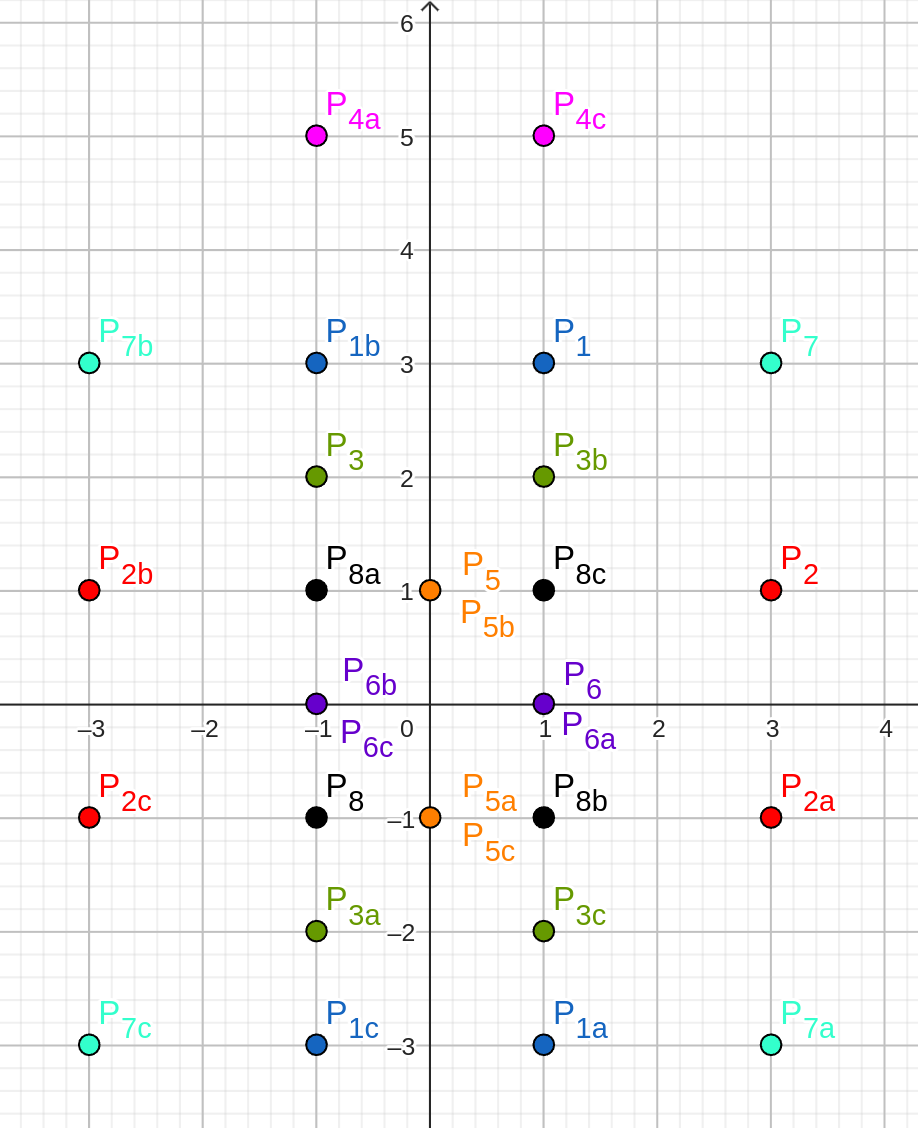
\includegraphics[scale=1]{../../common/sb_28/ex_00/ex_13.png} 
\centering
\label{fig:13}
\end{figure}

\end{document}
